%% The first command in your LaTeX source must be the \documentclass command.
%%
%% Options:
%% twocolumn : Two column layout.
%% hf: enable header and footer.
\documentclass[
% twocolumn,
% hf,
]{ceurart}

%%
%% One can fix some overfulls
\sloppy
\usepackage{graphicx}
\usepackage{textgreek}
\usepackage{enumitem}
%%
%% Minted listings support 
%% Need pygment <http://pygments.org/> <http://pypi.python.org/pypi/Pygments>
\usepackage{listings}
%% auto break lines
\lstset{breaklines=true}

%%
%% end of the preamble, start of the body of the document source.
\begin{document}

%%
%% Rights management information.
%% CC-BY is default license.
\copyrightyear{2025}
\copyrightclause{Copyright for this paper by its authors.
  Use permitted under Creative Commons License Attribution 4.0
  International (CC BY 4.0).}

%%
%% This command is for the conference information
\conference{OCL 2025 at STAF 2025,
 10 - 13 June 2025 Koblenz, Germany}

%%
%% The "title" command
\title{OCL Collection Optimization - Part 2 - Components}

%%
%% The "author" command and its associated commands are used to define
%% the authors and their affiliations.
\author[1,2]{Edward D. Willink}[%
orcid=0000-0003-3124-4019,
email=ed@willink.me.uk,
]
\cormark[1]
\fnmark[1]
\address[1]{Willink Transformations Ltd, Reading England}
\address[2]{Eclipse Foundation}



%%
%% The abstract is a short summary of the work to be presented in the
%% article.
\begin{abstract}
Collections and iterations provide much of the power of OCL. The apparent similarity of OCL's Set and Sequence to Java's Set and List encourages an OCL implementer to re-use the Java functionality. However OCL and Java are not the same. The immutability of OCL Collections can result in inefficient churning of intermediate results. We revisit the implementation of collections to provide determinism at no-cost, and identify a new characterization of iterations that supports compile-time optimizations.
\end{abstract}

%%
%% Keywords. The author(s) should pick words that accurately describe
%% the work being presented. Separate the keywords with commas.
\begin{keywords}
  OCL\sep
  Collection optimization \sep
  Iteration optimization
\end{keywords}

%%
%% This command processes the author and affiliation and title
%% information and builds the first part of the formatted document.
\maketitle

\section{Introduction}

OCL \cite{OCL-2.4} evolved to satisfy UML's \cite{UML-2.5} need for textual model constraints where graphics was not appropriate. When Eclipse OCL was used to rectify the very many problems \cite{wilke2011uml} in the pre-UML-2.5 OCL, UML's OCL was executed for the first time. Previous execution by commercial UML tools had been based on a manual transliteration with appropriate caches and fixes . The results for direct automated execution were very very disappointing. After some crazy speed problems were fixed, one significant remaining concern seemed to be the cost of cascades of collection operations.

"Deterministic Lazy Mutable OCL Collections" \cite{willink2017deterministic} reported on some attempts to improve collection performance. The mutable collections improved \verb!iterate! accumulation from O(N*N) to O(N). A unified deterministic collection showed promise but failed because the unified collection had no collection kind and so could use the wrong semantics for e.g. \verb!=! (equals). Lazy execution was difficult to achieve without unwanted incompatibilities.

In this paper we apply an extra level of indirection \cite{lampson1993principles} to make a unified deterministic collection feasible.  We also re-specify iterations without using iterate. This paves the way for part 3 of this paper to exploit laziness.

%Unfortunately early tooling was either of insufficient quality or not used and so the OCL constraints that formed part of UML models prior to UML 2.5 contained hundreds of errors. This provided a fruitful target for academic critique.

%For UML 2.5 \cite{UML-2.5}, Eclipse OCL \cite{Eclipse-OCL} was used to remove all syntactical errors such as mismatched parentheses or the use of the OCL 1 Enumeration Literal syntax and nearly all semantic errors such as inappropriate operators or operations. The extensive corpus of constraints also diagnosed faults in Eclipse OCL that once resolved identified further semantic errors. Four semantic errors were identified too late for correction of the UML 2.5 models. 

%No functional exercising of the OCL constraints took place. Rather each UML vendor manually transcribed the OCL into Java implementations for their tools. Very little feedback in terms of syntactic, semantic or functional errors was reported to the OMG, so the number of functional errors remains unknown.

%During development of Eclipse OCL's Validity View, UML's OCL constraints were accidentally used directly on the UML metamodel. Execution at least started, but took far too long to make any useful observations of the utility of the constraints. Investigation of the unacceptable speed diagnosed that the problem concerned long cascades of collection operations giving very high order execution times. The manual transcriptions and caches of real UML tools avoids the high orders. OCL tooling clearly needs improving to emulate what manual implementations were doing. 

In this part we first review typical collection implementations in Section~\ref{Collections}. Then in Section~\ref{CoCollections} we present a revised approach that offers better prospects for optimization. In Section~\ref{Iterations}, we re-specify iterations in a manner that suits implementation. The comparative performance of our new approach is presented in Section~\ref{Results}. In Section~\ref{Related Work} we report on related work and in Section~\ref{Summary} we summarize.

\section{Collections}\label{Collections}

The current OCL specification defines four concrete implementations of the abstract \verb!Collection! class. 
These support the four permutations of unique/non-unique, ordered/not-ordered content\footnote{Discussion following Gogolla \cite{gogolla2021refactoring} agreed on count-aware/count-blind and order-aware/order-blind as clearer terminology.}.

OCL tools implemented using Java of course seek to re-use Java types, so a typical implementation of the four specified kinds is summarized in Table \ref{tab:TypicalOCLCollection}.

\begin{table}[h]
\begin{tabular}{ c | c | c }
Specified Kind & Implementation Class & Contents \\
\hline
Sequence &  enhanced Java List & Array of elements \\
Set &  enhanced Java Set & Hashtable of elements \\
OrderedSet & adjusted Java LinkedHashSet & Hashtable of elements with linked list \\
Bag &  custom Bag using Java Map & Map of element value to occurrence count \\
\end{tabular}
\caption{Typical OCL Collection implementations}
\label{tab:TypicalOCLCollection}
\end{table}

The \verb!Sequence! and \verb!OrderedSet! forms provide for the obvious cases of creation/load-ordered content that may or may not be unique\footnote{Gogolla \cite{gogolla2019keynote} has suggested that consistent 3-letter names such as Seq and Ord would be more readable.}.

The additional \verb!Bag! and \verb!Set! forms allow the metamodeler to specify that order is not significant.

Unfortunately, OCL 1 did not provide the \verb!OrderedSet! type and so for many years \verb!Set! was used instead. This imposed a loss of ordering and introduced non-determinacy, which is a very strange attribute of an otherwise strong language. OCL 2 provided \verb!OrderedSet! without tackling the indeterminacy is OK culture.

From an implementation perspective, re-using Java's non-determinate HashSet is convenient and trades the loss of `irrelevant' order for a much faster implementation of includes/contains content testing. This is a bad trade-off since, at best, the indeterminacy can make debugging difficult. At worst, an unjustified confidence that ordering is not significant may lead to unpredictable failures. A different implementation of \verb!Set! could usefully preserve the creation / load ordering and, as we shall see, may actually be more efficient.

\verb!Bag! is perhaps the least useful of the collections. It is the inevitable result of a collection of not necessarily unique results derived from a set of elements. Traditional Java provides no counterpart for OCL's bag, so a bespoke implementation is necessary. This will probably provide a fast \verb!Bag.count()!. However, this operation is often not used, so the effort to provide eager support is dubious.

\subsection{Uniqueness / Count-awareness}

The uniqueness of elements provided by an \verb!OrderedSet! or \verb!Set! is of course important to avoid duplicate results. However, uniqueness is potentially expensive since creation of a set incurs an at least O(NlogN) cost rather than O(N) for a \verb!Sequence!. However, once this creation cost has been incurred, operations such as \verb!includes! compute in O(1) rather than O(N) time. A Java Set has no knowledge of how it will be used, so it makes the sensible trade-off to bound creation cost at O(NlogN) and testing at O(1) using a sophisticated memory expensive approach. As we shall see in Section~\ref{Results}, for at least small collections, a low-overhead representation may outweigh the correspondingly slower O(N*N) and O(logN) performance. 

\subsection{Order-awareness}

The ordering of elements in a collection may also be important and fundamental. For instance, a person's first, second, third, ... names are clearly ordered. So we use \verb!OrderedSet! or \verb!Sequence! kinds. 

Sometimes an order is useful but derived. For instance, houses may have one positional order for a postman's round or a second alphabetical order within a find-address-popup-menu. These two derived orders may differ from a third more fundamental  order associated with internal database entries. The internal order should not be exposed to the user, so specification of a \verb!Set! of houses is appropriate even though the underlying implementation has an order. In practice, all collections have an order that is defined by the order of creation or loading of model elements. Behind the scenes all collections can be ordered. \verb!Set! can be used to prevent OCL expressions exploiting the private implementation order, rather than being an excuse for indeterminacy. The private order is of course exposed by iterations. 

\section{CoCollections}\label{CoCollections}

Java collections are designed to support frequent mutation by operations such as \verb!Collection.add()!. The consumer of a Java Set is a Java program whose hard-to-analyze side-effects make it very difficult to tailor performance to the usage. Java therefore provides a good general purpose implementation that avoids over-complex derived state. (Derived state could accelerate rare operations but penalize common operations with incremental update costs.)

In contrast, OCL collections are immutable; each operation such as \verb!Collection.including()! results in a new collection. The consumer of an OCL collection is a side-effect-free OCL expression. The usage context can be exploited and since the final state of the collection is known, derived state can be eagerly or lazily computed and cached once; no incremental update will be required. Operations such as \verb!count! or \verb!includes! are applicable to all collection kinds and can benefit from a fast lookup.


\begin{table}[ht]
\begin{tabular}{ c | c }
Specified Kind & Implementation Classes \\
\hline
Sequence & Sequence view, CoCollection  \\
Set & Set view, CoCollection \\
OrderedSet & OrderedSet view, CoCollection \\
Bag & Bag view, CoCollection \\
\end{tabular}
\caption{Revised OCL Collection implementations with CoCollections}
\label{tab:RevisedOCLCollection}
\end{table}

We therefore propose to replace the four heavyweight classes for each collection kind, by four lightweight view classes that delegate to a unified \verb!CoCollection! as shown in Table~\ref{tab:RevisedOCLCollection}. As indicated in Figure~\ref{fig:CoCollectionContents}, the \verb!CoCollection! holds the \verb!elements! of a collection in a fixed-sized ordered array of not-necessarily unique elements, thereby directly supporting a \verb!Sequence! and the \verb!->asSequence()! `conversion'. Other kinds and `conversion's are supported by additional lazily computed contents.

%An example of derived state is provided by the value-to-count map that underpins a bag or a fast \verb!Collection.includes()! operation.

When unique behavior is required, the optional \verb!isFirst! is computed so that a unique iteration of a \verb!CoCollection! skips the non-\verb!isFirst! elements that duplicate earlier indexes. We may therefore rewrite \verb!aSequence->asSet()->forAll(p | ...)! as:

\begin{description}[itemsep=-0.2cm]\vspace{-10pt}\small\begin{samepage}
\item \verb!let coCollection = aSequence->coCollection() in!
\item ~~~~\verb!coCollection.elements->forAll(p | coCollection.isFirst(p) implies ...)!
\end{samepage}\vspace{-10pt}\end{description}

The \verb!isFirst! bit array can be efficiently computed from the \verb!hash2index! `map'. The `map' is realized as an array of entries from each element's hashcode to its index within the \verb!elements! array. The entries are sorted in hashcode order. A binary search can therefore locate the index of an element via its hashcode for an  \verb!includes! operation in O(logN) time. Duplicate entries have duplicate hashcodes in adjacent entries, so the \verb!count! operation counts all adjacent entries whose index identifies the element of interest. Significant speed-up of \verb!intersection! is possible as we shall see in Section~\ref{Results}, where the performance of variants of the \verb!CoCollection! approach optimized for diverse collection sizes are contrasted with a Java HashSet approach.

%entries that `map' an element's hashcode to the element's index within the \verb!elements! array. The `map' is persisted within the \verb!CoCollection! since it is useful for value queries such as \verb!includes! or \verb!count!. A binary search for the value's hashcode locates the first index. An iteration over adjacent entries can count duplicates. The array of entries gives substantial size savings compared to a regular Java Map. A binary search of the entries gives small speed improvements too for small collections. Significant speed improvements are possible for an intersection.

\begin{figure}[b]
	\vspace{-10pt}
	\begin{center}
		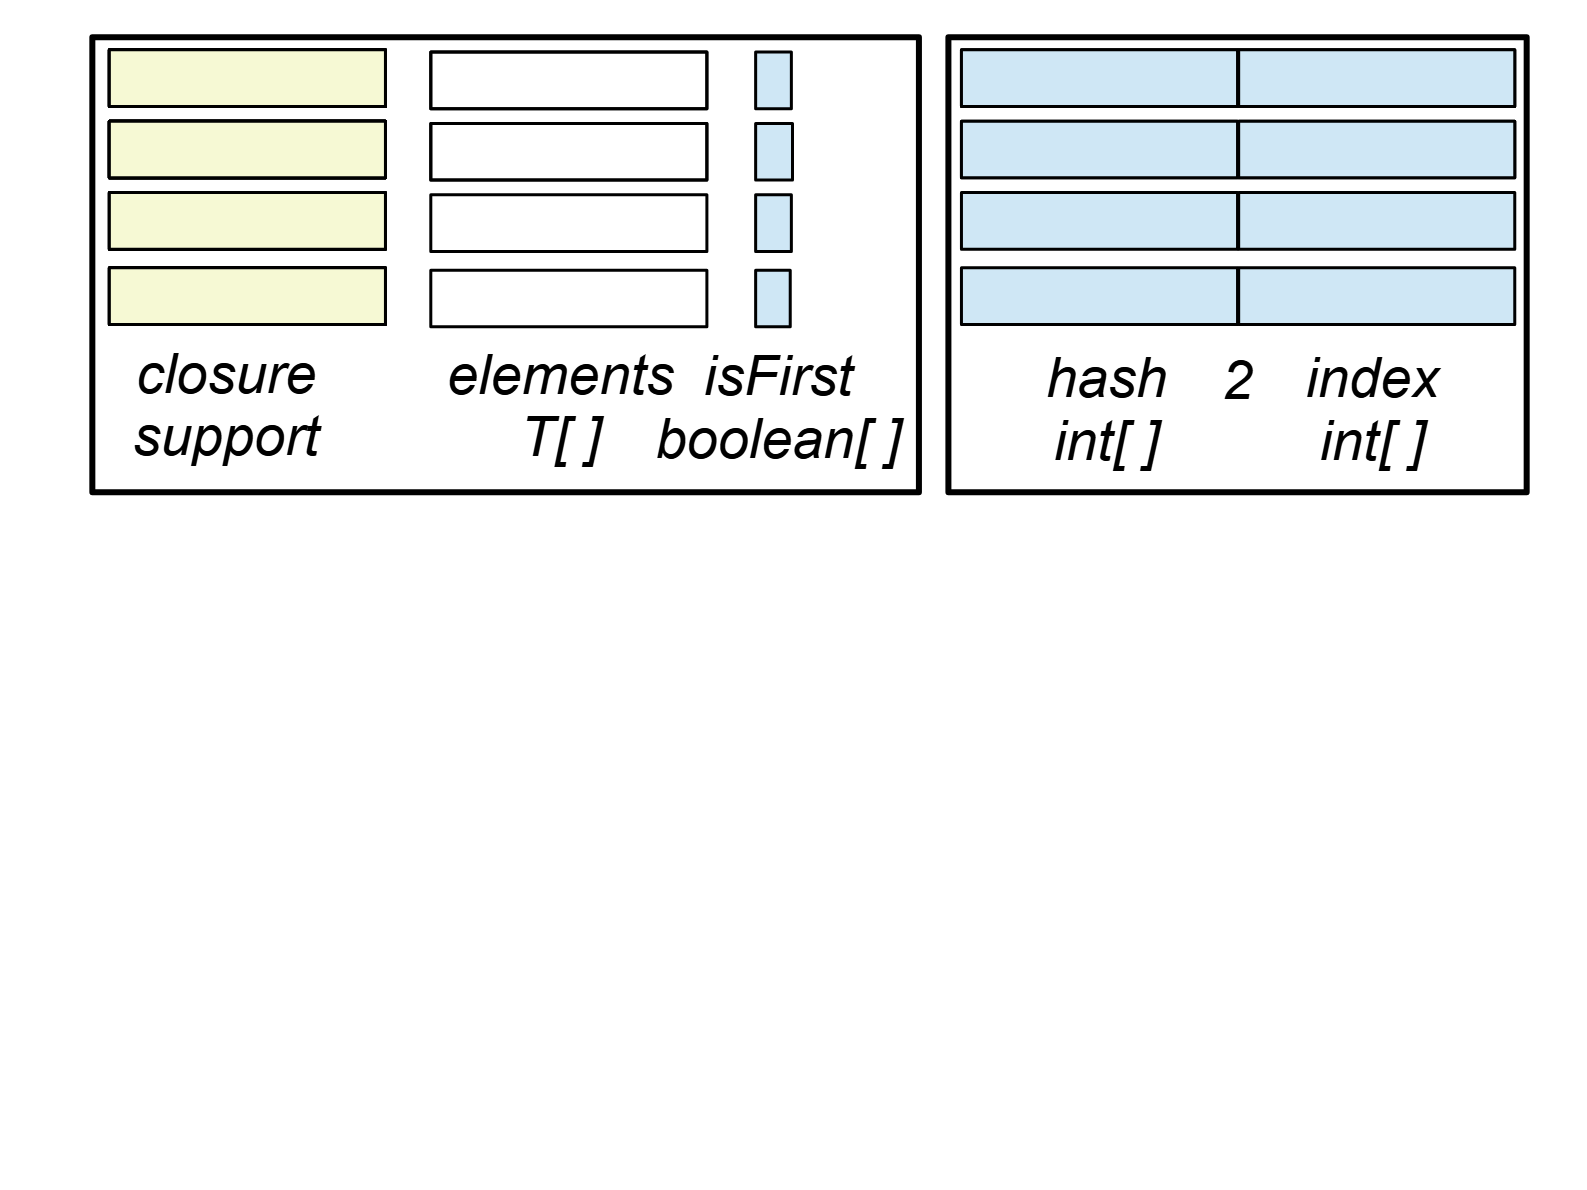
\includegraphics[trim= 0 340 0 0,clip,width=5.0in]{CoCollection.png}
	\end{center}
	\vspace{-10pt}
	\caption{CoCollection arrays}
	\label{fig:CoCollectionContents}
	\vspace{-10pt}
\end{figure}

% Figure~\ref{fig:CoCollectionContents} shows that additional caching may be provided for specialized usages such as \verb!closure!.

%With the exception of the \verb!elements! array, the other contents are computed lazily. Many usages such as a set-iteration mandate creation of the lazy cache, however some usages such as a \verb!count! of a \verb!Sequence! do not. A simple heuristic such as whether the \verb!count! is used within a loop can decide whether to use a cached or uncached computation.

%When required, the \verb!hash2index! mapping is established by populating each entry with each element's hashcode and \verb!elements! array index. Once the entries are sorted into hash order, the \verb!hash2index! may be accessed by binary search to locate the first index of each value. 

%Whereas in \cite{willink2017deterministic}, we advocated a unified Collection class always comprising an \verb!ArrayList! and lazily expanding to a \verb!HashSet! when required we now advocate, as shown in \ref{fig:CoCollectionContents} a fixed size array for the elements. This is all that is needed for the \verb!Sequence! view. When uniqueness is required, the addional index-correlated \verb!isFirst! array of \verb!boolean!s identifies those elements that have no preceding equal value. Efficient computation of \verb!isFirst! can exploit a sort of the elements' hash values. When required, the \verb!hash2index! mapping is established by populating each entry with the each element's hashcode and \verb!elements! array index. Once the entries are sorted into hash order, the \verb!hash2index! may be accessed by binary search to locate the first index of each value. Duplicate entries can be counted in adjacent entries. Binary-search using an array is more efficient and much smaller than a hash tree for small collections. Since the \verb!CoCollection! is hidden, an alternate hash tree implementation can be used for large collections. Similarly optimised \verb!EmptyCoCollection!, \verb!SingletonCoCollection! and \verb!TinyCoCollection! can support the common use cases of really small collections.

%Once the collection functionality has been unified and hidden, we can polymorphize it with specialized \verb!EmptyCoCollection!, \verb!SingletonCoCollection!, \verb!TinyCoCollection!, \verb!SmallCoCollection! and \verb!LargeCoCollection! for perhaps 0, 1, 2-4, 5-256, 257-... elements and no/check/linear/binary/hashed search strategies respectively.


On a modern 64-bit computer, the size of a sequence-only \verb!CoCollection! is 8 bytes per element; just the same as a Java ArrayList. Once the lazy set-functionality is activated, the size grows to 17 bytes per element, significantly less than about 36 bytes per element for Java HashSet or 44 bytes for a deterministic Java variant of HashSet. A further lazy growth can support sharing of partial \verb!closure! results for the common use case where overlapping closures are computed for many elements of a collection.

Whether the lazy growth is worthwhile can be subject to heuristics observing whether usage of \verb!count! within an iteration loop is likely to benefit from re-use whereas an isolated use of \verb!count! may be better realized as a naive linear traversal.

%With the exception of the \verb!elements! array, the other contents are computed lazily. Many usages such as a set-iteration mandate creation of the lazy cache, however some usages such as a \verb!count! of a \verb!Sequence! do not. A simple heuristic such as whether the \verb!count! is used within a loop can decide whether to use a cached or uncached computation.

%Table~\ref{tab:CoCollectionCaches} identifies some lazy caches that may be populated by an operation execution. In the absence of detailed profiling, whether to create a cache must be determined by heuristics. The simplest heuristic caches for an operation within an iteration loop where the cache is likely to be beneficial. Conversely, where an operation occurs in isolation, the caching cost is probably unjustified. When more detailed analysis can predict loop counts or count multiple isolated operations a tighter heuristic can be employed.

%\begin{table}[ht]
%\begin{tabular}{ c | c | c }
%Operation & Caching \\
%\hline
%asSet & isFirst(x) bit array identifying unique elements \\
%count, includes, indexOf & hash-sorted array of value-to-index entries \\
%closure & map of partial closures \\
%\end{tabular}
%\caption{CoCollection Cached Analyses}
%\label{tab:CoCollectionCaches}
%\end{table}

%Since the \verb!CoCollection! is hidden from the OCL author, its implementation  can be flexible. Most models have quite small, sometimes very small, collections so that linear algorithms or a binary search can be optimum. On those rare occasions where a huge collection is in use, an alternate \verb!CoCollection! implementation can change gears and use hash tables.

%It must be stressed that while this paper `starts again' with respect to collection implementation, it does not make any changes to what the OCL author may write. The rewrites presented in this paper represent rewrites that an OCL tool may perform behind the scenes in order to provide improved performance of the author's unchanged intent.

%\subsection{Sequence}

%In our new approach, \verb!Sequence! is the fundamental kind of collection. The  \verb!Sequence! comprises an array of the collection elements with a known size and type. The array provides a deterministic order and fast access via the \verb!at! operation. A \verb!Sequence! has no need for the extra \verb!CoCollection! caches, but they  may be created if looped usage of an operation such as \verb!includes! or \verb!indexOf! justifies a hash-to-index cache.

%\subsection{OrderedSet}

%We support an \verb!OrderedSet! as the basic \verb!Sequence! with an additional `mask' to inhibit usage of repetitions of earlier elements. This mask of `isFirst' values is hosted by the \verb!CoCollection! using an array of Boolean values at matching indexes; a true value identifies the first occurrence of each value and a false value a repeated occurrence. This extra array may be interrogated by the \verb!CoCollection.isFirst!  operation. We may therefore rewrite \verb!aSequence->asSet()->forAll(p | ...)! as:

%\begin{description}[itemsep=-0.2cm]\vspace{-10pt}\small\begin{samepage}
%\item \verb!let coCollection = aSequence->coCollection() in!
%\item ~~~~\verb!aSequence->forAll(p | coCollection.isFirst(p) implies ...)!
%\end{samepage}\vspace{-10pt}\end{description}

%The let-variable reifies the empty \verb!CoCollection! as an explicit variable where Common Subexpression Elimination may contrive to share diverse usages. The first invocation of  \verb!isFirst! triggers the lazy computation of the repetition guards that ensure that only the first values are used by the loop. Efficient detection of duplicates can be provided by sorting an array of value-to-index entries. The value-to-index cache may be created as a precursor.

%This rewrite trades the reification of a set of elements for the lazy creation of a matched-index array of Booleans. The latter requires less memory and provides better opportunities for sharing amongst diverse computations.

%The same array value-to-index entries that lazily supports a fast \verb!includes! or \verb!indexOf! for \verb!Sequence! may of course support \verb!OrderedSet! as well. (Multiple indexes for the same value can use adjavent entries.)

%\subsection{Set}

%Once we enforce determinacy, there is no internal difference between a \verb!Set! and an \verb!OrderedSet!; \verb!Set! is redundant. The user's specified distinction is of course maintained to provide type checking that may alert the user to the unexpected imposition of an ordering.

%\subsection{Bag}

%An implementation of a \verb!Bag! could maintain a repeat count of each value and so reduce the required memory to represent all values.  For large \verb!Bag!s and where the count is used, the saving can be worthwhile. However the count is often not used.

%Rather than saving memory, a \verb!Bag! is more often the fallback type for intermediate results whose ordering and uniqueness have been lost. The effort to count elements is therefore often wasted. Iteration over a \verb!Bag! repeats the counted elements giving no performance benefit from the repeat count.

%When actually needed, the repeat count can be lazily computed and persisted as an array of value-to-count entries in the \verb!CoCollection! rather than the \verb!Bag!. Thus \verb!s->count(x)! can be rewritten as:
%\begin{description}[itemsep=-0.2cm]\vspace{-10pt}\small\begin{samepage}
%\item \verb!let coCollection = s->coCollection() in!
%\item ~~~~\verb!coCollection.count(x)!
%\end{samepage}\vspace{-10pt}\end{description}

%This rewrite exposes the \verb!coCollection! for sharing. The lazily cached array of value-to-count entries is available to support fast response of \verb!excludes! or \verb!includes! as well as \verb!count! for all collection kinds.

%Behind the scenes, the \verb!Bag! type is redundant even though it is a useful part of the type system presented to the user.

\subsection{Redundant Uniqueness}

A further speed trade-off is available for the \verb!aSequence->asSet()->forAll(p | ...)! rewrite when the cost of the loop body \verb!...! is smaller than the \verb!coCollection.isFirst(p)! repetition guard. The guard can be omitted since neglecting to prune duplicate \verb!forAll! terms does not change the result. We can rewrite as \verb!aSequence->forAll(p | ...)! omitting the \verb!->asSet()!. The small cost of \verb!coCollection.isFirst(p)! is known. If we can confidently estimate the cost of \verb!...!, the appropriate trade-off is possible.

Since OCL is side effect free, we can commute uniqueness enforcement with other computations so that the following are all equivalent:

\begin{description}[itemsep=-0.2cm]\vspace{-10pt}\small\begin{samepage}
\item \verb!aCollection->asSet()->select(...)->asSet()!
\item \verb!aCollection->select(...)->asSet()->asSet()!
\item \verb!aCollection->select(...)->asSet()!
\end{samepage}\vspace{-10pt}\end{description}

The latter saves the cost of a set enforcement but again incurs the additional cost of a redundant \verb!select(...)! for each repeated element. Whether this is a good trade off cannot be accurately determined at compile time without profiling information. However, the cost of \verb!select(...)! can be estimated heuristically at compile time. Combined with knowledge of the collection size at run-time, a plausible eager/lazy trade-off can be achieved.

\subsection{Explicit indexOf}

The simple implementation of \verb!indexOf! for an \verb!OrderedSet! or \verb!Sequence! involves a linear search of typically half the content to locate the matching value; O(N).

This can be accelerated dramatically using the \verb!CoCollection!'s sorted array of \verb!hash2index! entries. The O(N) linear-search can therefore be replaced by the much faster binary search; O(logN). The size of the entry array is also significantly smaller than a full map.

\subsection{Implicit indexOf}

A common use of \verb!indexOf! occurs when correlating two lists such as the parameter and argument lists of an operation call. The iteration over one list provides one element (parameter) whose index is used to locate the corresponding second element (argument). In the following \verb!f(par, arg)! performs the correlation check.

\begin{description}[itemsep=-0.2cm]\vspace{-10pt}\small
\item ~~~~~~~~\verb!pars->forAll(par | let arg = args->at(pars->indexOf(par)) in f(par, arg))!
\vspace{-10pt}\end{description}

The inefficiency of this is offensive; why is a content search necessary to discover the index that the iteration already knows? Eclipse OCL supports a coIterator \cite{willink2019map} that provides the index of a list iteration (or the value of a map iteration).

\begin{description}[itemsep=-0.2cm]\vspace{-10pt}\small
\item ~~~~~~~~\verb!pars->forAll(par with index | let arg = args->at(index) in f(par, arg))!
\vspace{-10pt}\end{description}

(The \verb!with! keyword separates the regular iterator \verb!par! from its coIterator \verb!index!.)

Avoiding the unnecessary \verb!indexOf! call may avoid the need to populate the \verb!CoCollection! \verb!hash2index! cache that provides the \verb!indexOf! support.

%\subsection{Safe OCL} XXXX ???

%OCL is specified to be functional and side-effect-free. An OCL expression once parsed to its Abstract Syntax Tree form observes Static Single Assignment policies and so optimizations such as Constant Folding, Common Subexpression Elimination, Loop Hoisting and Inlining are straightforward.

%Two phenomena undermine the ideality of the specification.

%UML permits an operation to be defined as not-a-query; ie. side-effecting. This is not safe. A pedantic OCL tool may simply refuse to execute. More usefully all optimisations may be suppressed so that execution may correspond to a user expectation.

%OCL permits an operation such as \verb!at! to crash for a bad-index. The divide operation fails for divide by zero. More generally a navigation with a null source fails.For Java, we are familiar with exceptions that propagate until caught. OCL is in many ways similar, \verb!invalid! propagates until `caught' by an \verb!oclIsInvalid()! call. Unfortunately the \verb!and!/\verb!or! operations are specified to be mathematically pure; they are commutative. In contrast most languages define \verb!and!/\verb!or! to be short-circuit so that a crash on the first term obviates computation of the second. In OCL, if the first term crashes, evaluation of the second term may `uncrash' the computation; the result of \verb!crash and false! is \verb!false! rather than \verb!crash!. A detailed expression analysis may be able to statically prove that one of the terms cannot crash and rewrite to compute the safe term first. Where both terms are not safe the expression is unsafe.

%Safe OCL applies to the subtrees of the AST in which there are no side effects and no uncrashing. These subtrees can be optimized. The remainder of the %AST cannot be optimized. The optimizations in this paper assume we are considering a safe OCL subtree.

\section{Iterations}\label{Iterations}

The generic \verb!iterate! iteration is specified in OCL 2.4 \S11.8 as the basis for all iterations. 

\begin{quote}\textit{
The semantics of each iterator expression is defined through a mapping from the iterator to the ‘iterate’ construct. %This means that the semantics of the iterator expressions do not need to be defined separately in the semantics sub clauses.
}\end{quote}

Emulating the definition-rewrite as an implementation-rewrite to use \verb!iterate! can be a poor basis for tooling. Consider \verb!aCollection->collect(p | ...)! where \verb!aCollection! is a collection of \verb!T!-typed elements and \verb!...! is the lambda-expression for the loop body . It may be rewritten as:

\begin{description}[itemsep=-0.2cm]\vspace{-10pt}\small
\item ~~~~~~~~\verb!aCollection->iterate(p; acc = Bag(T){} | acc->includes(...))!
\vspace{-10pt}\end{description}

This is very inefficient since each sequential per-element update of the accumulator creates a new collection. The overall performance will be O(N*N) for count-blind and O(N*N*logN) for count-aware collections. A more efficient direct implementation can exploit the invisibility of \verb!acc! outside of the iteration and so use a hidden mutable Java collection \cite{willink2017deterministic}. This can improve performance to O(N) for count-blind and O(N*logN) for count-aware collections. %The option of a concurrent multi-processor solution is shut out by \verb!iterate!.

\verb!iterate! semantics are too strong for the procedural \verb!any!, \verb!exists!, \verb!forAll!, \verb!isUnique! and \verb!one! iterations that must proceed sequentially, but which may terminate early; `iterate' does not allow for early termination.

\verb!iterate! semantics are too strong for the declarative \verb!closure!, \verb!collect!, \verb!collectNested!, \verb!reject!, \verb!select! and \verb!sortedBy!  iterations that may execute concurrently; `iterate' does not allow for concurrency.

We therefore introduce a new characterization of OCL iterations by rewriting to one of two new underlying iterations, a helper operation and a special place-holdingvalue.

\subsection{Declarative gathers}

The new \verb!gather! iteration gathers the results of a per-element lambda-expression to form a new collection. It is identical to \verb!collectNested! but fundamental,  rather than a remedy for the pragmatic \verb!collect!. The \verb!Sequence! overload of \verb!gather! is modelled using the Eclipse OCL standard library \cite{willink2011modeling} as:

\begin{description}[itemsep=-0.2cm]\vspace{-10pt}\small\begin{samepage}
\item \verb!type Sequence(T) : SequenceType conformsTo OrderedCollection(T)!
\item  \verb!{!
\item ~~~~\verb!iteration gather(V)(i : T[?] | lambda : Lambda T() : V[?]) : Sequence(V) {!
\item ~~~~~~~~\verb!post: self->forAll(i with x | result->at(x) = i.lambda());!
\item ~~~~\verb!}!
\end{samepage}\vspace{-10pt}\end{description}
\begin{description}[itemsep=-0.2cm]\vspace{-10pt}\small\begin{samepage}
\item ~~~~\verb!iteration collectNested(V)(i : T[?] | lambda : Lambda T() : V[?]) : Sequence(V) {!
\item ~~~~~~~~\verb!body: self->gather(i | i.lambda());!
\item ~~~~\verb!}!
\end{samepage}\vspace{-10pt}\end{description}
\begin{description}[itemsep=-0.2cm]\vspace{-10pt}\small\begin{samepage}

\item ~~~~\verb!iteration select(i : T[?] | lambda : Lambda T() : Boolean[1]) : Sequence(T) {!
\item ~~~~~~~~\verb!body: self->gather(i | if i.lambda() then i else! $\omega$ \verb!endif)->compact();!
\item ~~~~\verb!}!
\end{samepage}\vspace{-10pt}\end{description}
\begin{description}[itemsep=-0.2cm]\vspace{-10pt}\small\begin{samepage}
\item ~~~~\verb!operation compact() : Sequence(T) {!
\item ~~~~~~~~\verb!post: result->excludes(!$\omega$\verb!);!
\item ~~~~\verb!}!
\item \verb!}!
\end{samepage}\vspace{-10pt}\end{description}

The collection class template parameter \verb!T! and iteration template parameter \verb!V! define the type signature. \verb!gather! has a single iterator \verb!i! whose type corresponds to the source collection element type; it may be null. The iteration body is modeled as a lambda expression named \verb!lambda! and typed as a \verb!Lambda! from a \verb!T! source without parameters to a \verb!V! return that may be null. The iteration result is a \verb!Sequence(V)!.

%The postcondition uses the Eclipse OCL coValue extension for iterators. The \verb!with! keyword introduces the coValue \verb!x!, which is a secondary iterator whose value is \verb!self->indexOf(i)!\footnote{Not quite. For a non-unique sequence, indexOf returns the first index; the coVolue increases monotonically.}. 

The postcondition specifies that the result is element-wise the result of computing the lambda expression for the input element.

The \verb!collectNested! rewrite is trivial; functionality is delegated directly to \verb!gather!. 

The specification of \verb!select! once again has a source-typed iterator \verb!i!, and a lambda-expression that is now required to have a \verb!Boolean! result. The \verb!body! defines an implementation of the iteration that rewrites to the \verb!gather! iteration with a nested lambda-expression that wraps the selection in an \verb!if!. The \verb!if! variously selects the wanted \verb!i! or the unwanted $\omega$.

The $\omega$ special value is a place-holding collection element for a collection element that is not-available. It is intentionally missing; there is nothing \verb!invalid! or \verb!null! about $\omega$. Any computation using $\omega$ is not-available, since $\omega$ should have been optimized away.  $\omega$ is a compile-time artifice to ensure that the \verb!gather! result is the same-size as its source. In part 3 \cite{Willink-Collections3} this facilitates \verb!gather!-\verb!gather! optimizations.

The \verb!compact! helper operation converts a collection that may involve not-available $\omega$ values to a regular collection without these values. Higher index elements are moved down to eliminate the gaps.

The \verb!collect! iteration, not shown, appends a \verb!flatten! call to the \verb!collectNested! rewrite. Most usages of \verb!collect! do not use nested collections and so the redundant \verb!flatten! can be omitted.

The \verb!reject! rewrite, not shown, is  similar to \verb!select!. It just swaps \verb!then! and \verb!else! terms.

%The shape of the result mirrors that of the input with excluded output elements from \verb!reject! or \verb!select! accomodated by the new not-available $\omega$ special value. A \verb!x->reject(p | f(p))! iteration call using the \verb!f(p)! lambda-expression may be rewritten as:

%\begin{description}[itemsep=-0.2cm]\vspace{-10pt}\small
%\item  \verb!x->gather(p | if f(p) then! $\omega$ \verb!else p endif)->compact()!
%\vspace{-10pt}\end{description}

\subsection{Procedural searches}

The new \verb!search! iteration supports the \verb!any!, \verb!exists!, \verb!forAll!, \verb!isUnique! and \verb!one! iterations. The traditional \verb!iterate! supports one iterator, one intermediate result accumulator and one lambda-expression for the next-accumulator-value update. The semantics are informal. The new \verb!search! supports multiple iterators with two additional lambda-expressions. The semantics are defined using a postcondition. The additional \verb!break! lambda-expression determines whether the iteration can terminate early. The additional \verb!return! lambda-expression determines the return value. The result type may therefore differ from the accumulator type as required by the \verb!one! iteration.

The one-iterator variants of \verb!search!, and the rewrite from \verb!exists!, are modeled using the Eclipse OCL standard library language as:

% with perhaps multiple iterators, an accumulator for the intermediate result and three lambda-expressions; one for the accumulator update, one to determine when to terminate and a third to provide the return. the \verb!x->exists(i, j, k | f(i, j, k))!  iteration call in which \verb!f(i, j, k)! is the lambda-expression body using the three iterators\footnote{Triple iterators were introduced by USE OCL}. This may be rewritten\footnote{elseif is a rather obvious syntax sugar supported by Eclipse OCL:.}

%The \verb!search! iteration like \verb!iterate! processes each input element sequentially with an iterator, accumulator and lambda-expression to determine the next accumulator value. Syntactically they are separated by \verb!;! and then \verb!|!. \verb!iterate!'s limitations on early exit, and the requirement for the accumulator to be the result are removed by defining two further lambda-expression arguments. \verb!isDone! is true for the search to terminate early. \verb!result! is the value to be returned. To accommodate this flexibility, the iteration requires distinct operation template parameters \verb!V! and \verb!W! for result and accumulator types respectively, in addition to the outer class template parameter \verb!T! for the collection element type.

\begin{description}[itemsep=-0.2cm]\vspace{-10pt}\small\begin{samepage}
\item \verb!type Sequence(T) : SequenceType conformsTo OrderedCollection(T)!
\item  \verb!{!
\item ~~~~\verb!iteration search(V,W)(i : T[?]; acc : W | next : Lambda W(T) : W, !
\item ~~~~~~~~~~~~~~~\verb!break : Lambda W(T) : Boolean, return : Lambda W(T) : V[?]) : V[?] {!
\item ~~~~~~~~\verb!post: let accs:Sequence(W), breaks:Sequence(Boolean), returns:Sequence(V) in!
\item ~~~~~~~~~~~~~~~~\verb!self->forAll(i with x |!
\item ~~~~~~~~~~~~~~~~~~~~~~~~\verb!let nextAcc = if x = 1 then acc else accs->at(x-1) endif.next(i) in!
\item ~~~~~~~~~~~~~~~~~~~~~~~~\verb!let nextBreak = nextAcc.break(i) in!
\item ~~~~~~~~~~~~~~~~~~~~~~~~\verb!accs->at(x) = if nextBreak then! $\omega$ \verb!else nextAcc endif! 
\item ~~~~~~~~~~~~~~~~~~~~~~~~\verb!and breaks->at(x) = nextBreak!
\item ~~~~~~~~~~~~~~~~~~~~~~~~\verb!and returns->at(x) = nextAcc.return(i)!
\item ~~~~~~~~~~~~~~~~\verb!) and result = if notEmpty() then returns->at(self->size())!
\item ~~~~~~~~~~~~~~~~~~~~~~~~~~~~~~~~~~~~~~~~~~~~~~~~~~~~\verb!else acc.return(null) endif;!
\item ~~~~\verb!}!
\end{samepage}\vspace{-10pt}\end{description}
\begin{description}[itemsep=-0.2cm]\vspace{-10pt}\small\begin{samepage}
\item ~~~~\verb!iteration exists(i : T[?] | lambda : Lambda T() : Boolean[?]) : Boolean[?] {!
\item ~~~~~~~~\verb!body: self->search(i; acc : Boolean[?] = false |!
\item ~~~~~~~~~~~~~~~~~~~~~~~~~~~~\verb!let e = i.lambda() in!
\item ~~~~~~~~~~~~~~~~~~~~~~~~~~~~\verb!if e = true then true!
\item ~~~~~~~~~~~~~~~~~~~~~~~~~~~~\verb!elseif acc.oclIsInvalid() then acc!
\item ~~~~~~~~~~~~~~~~~~~~~~~~~~~~\verb!elseif e.oclIsInvalid() then e!
\item ~~~~~~~~~~~~~~~~~~~~~~~~~~~~\verb!elseif acc = null then null!
\item ~~~~~~~~~~~~~~~~~~~~~~~~~~~~\verb!elseif e = null then null!
\item ~~~~~~~~~~~~~~~~~~~~~~~~~~~~\verb!else false endif,!
\item ~~~~~~~~~~~~~~~~~~~~~~~~~~~~\verb!acc = true,!
\item ~~~~~~~~~~~~~~~~~~~~~~~~~~~~\verb!acc);!
\item ~~~~\verb!}!
\end{samepage}\vspace{-10pt}\end{description}
\begin{description}[itemsep=-0.2cm]\vspace{-10pt}\small\begin{samepage}
\item ~~~~\verb!iteration one(i : T[?] | lambda : Lambda T() : Boolean[?]) : Boolean[?] {!
\item ~~~~~~~~\verb!body: self->search(i; acc : Integer = 0 |!
\item ~~~~~~~~~~~~~~~~~~~~~~~~~~~~\verb!if i.lambda() then acc + 1 else acc endif,!
\item ~~~~~~~~~~~~~~~~~~~~~~~~~~~~\verb!acc > 1,!
\item ~~~~~~~~~~~~~~~~~~~~~~~~~~~~\verb!acc = 1);!
\item ~~~~\verb!}!
\end{samepage}\vspace{-10pt}\end{description}
\begin{description}[itemsep=-0.2cm]\vspace{-10pt}\small\begin{samepage}
\item ~~~~\verb!operation compact() : Sequence(T) {!
\item ~~~~~~~~\verb!body: self->search(i; acc = Sequence{} |!
\item ~~~~~~~~~~~~~~~~~~~~~~~~~~~~~~~~~~~~~~~~\verb!if i =! $\omega$ \verb! then acc else acc->append(i) endif, false, acc);!
\item ~~~~\verb!}!
%\end{samepage}\vspace{-10pt}\end{description}
%\begin{description}[itemsep=-0.2cm]\vspace{-10pt}\small\begin{samepage}
%\item ~~~~\verb!operation compactingSize() : Integer {!
%\item ~~~~~~~~\verb!body: self->search(i; size : Integer = 0 |!
%\item ~~~~~~~~~~~~~~~~~~~~~~~~~~~~~~~~~~~~~~~~\verb!if i =! $\omega$ \verb! then size else size+1 endif, false, size);!
%\item ~~~~\verb!}!
%\end{samepage}\vspace{-10pt}\end{description}
%\begin{description}[itemsep=-0.2cm]\vspace{-10pt}\small\begin{samepage}
%\item ~~~~\verb!operation compactingSizeLessThan(sizeThreshold : Integer) : Boolean {!
%\item ~~~~~~~~\verb!body: self->search(i; size : Integer = 0 |!
%\item ~~~~~~~~~~~~~~~~~~~~~~~~~~~~~~~~~~~~~~~~\verb!if i =! $\omega$ \verb! then size else size+1 endif,!
%\item ~~~~~~~~~~~~~~~~~~~~~~~~~~~~~~~~~~~~~~~~\verb!size >= sizeThreshold, size < sizeThreshold);!
%\item ~~~~\verb!}!
\item \verb!}!
\end{samepage}\vspace{-10pt}\end{description}

The \verb!search! postcondition uses the artifice of uninitialized \verb!Sequence!s that serialize each of the intermediate results. Each uninitialized \verb!Sequence! element is `initialized' exactly once by constraining its value before it is used in a later iteration.

%The \verb!search! iteration supports \verb!any!, \verb!exists!, \verb!forAll!, \verb!isUnique! and \verb!one! iterations with perhaps multiple iterators, an accumulator for the intermediate result and three lambda-expressions; one for the accumulator update, one to determine when to terminate and a third to provide the return. the \verb!x->exists(i, j, k | f(i, j, k))!  iteration call in which \verb!f(i, j, k)! is the lambda-expression body using the three iterators\footnote{Triple iterators were introduced by USE OCL}. This may be rewritten\footnote{elseif is a rather obvious syntax sugar supported by Eclipse OCL:.}

%\begin{description}[itemsep=-0.2cm]\vspace{-10pt}\small
%\item \verb!x->search(i, j, k; acc : Boolean[?] = false |!
%\item ~~~~~~~~~~~~~~~~~~~~\verb!let x = f(i, j, k) in!
%\item ~~~~~~~~~~~~~~~~~~~~\verb!if x = true then true!
%\item ~~~~~~~~~~~~~~~~~~~~\verb!elseif acc.oclIsInvalid() then acc!
%\item ~~~~~~~~~~~~~~~~~~~~\verb!elseif x.oclIsInvalid() then x!
%\item ~~~~~~~~~~~~~~~~~~~~\verb!elseif acc = null then null!
%\item ~~~~~~~~~~~~~~~~~~~~\verb!elseif x = null then null!
%\item ~~~~~~~~~~~~~~~~~~~~\verb!else false endif,!
%\item ~~~~~~~~~~~~~~~~~~~~\verb!acc = true,!
%\item ~~~~~~~~~~~~~~~~~~~~\verb!acc)!
%\vspace{-10pt}\end{description}

The \verb!exists! rewrite has a complicated lambda-expression to support 4-valued Booleans: any \verb!true! returns \verb!true!, else any \verb!invalid! returns \verb!invalid!, else any \verb!null! returns \verb!null!, else \verb!false!. The second lambda-expression \verb!break!s when the accumulator is \verb!true!. The third lambda-expression returns \verb!true!, \verb!invalid!, \verb!null! or \verb!false!.

%The complexity of the first lambda expression is caused by the 4-valued Boolean OCL support for \verb!exists! for which any \verb!true! returns \verb!true! else any \verb!invalid! returns \verb!invalid! else any \verb!null! returns\verb!null! else \verb!false!.
The rewrite is much simpler when symbolic analysis is able to prove that \verb!i.lambda()! is 2-valued.

\begin{description}[itemsep=-0.2cm]\vspace{-10pt}\small
\item ~~~~~~~~\verb!x->search(i; acc : Boolean[1] = false | i.lambda(), acc, acc)!
\vspace{-10pt}\end{description}

\subsection{closure}

The \verb!closure! iteration does not fit the above characterization since an efficient implementation involves a hidden map \cite{willink2019map}. With the aid of the hidden map and using \verb!...! to represent the arbitrary lambda-expression, \verb!aCollection->closure(...)! may be rewritten as

\begin{description}[itemsep=-0.2cm]\vspace{-10pt}\small
\item ~~~~~~~~\verb!aCollection->gather(p | closureMap->at(p))->flatten()->asSet()!
\vspace{-10pt}\end{description}

The hidden map contains each of the required closure partial results. The map contents satisfy the following recursive constraint.

\begin{description}[itemsep=-0.2cm]\vspace{-10pt}\small\begin{samepage}
\item ~~~~~~~~\verb!closureMap->forAll(k with v |!
\item ~~~~~~~~~~~~~~~~~~~~~~~~\verb!v = v->gather(...)->gather(q | closureMap->at(q))->flatten()->asSet()!
\item ~~~~~~~~~~~~~~~~\verb!)!
\end{samepage}\vspace{-10pt}\end{description}

The value of each \verb!k,v! map entry is the (transitive) aggregation of the map entries. 

The hidden map(s) may be cached as part of the \verb!CoCollection! to avoid re-computation when the \verb!closure! is re-used with the same lambda-expression.

\subsection{sortedBy}

Evaluation of \verb!aCollection->sortedBy(k | f(k))! similarly involves creation of a hidden map from sort key to original element.

\begin{description}[itemsep=-0.2cm]\vspace{-10pt}\small\begin{samepage}
\item ~~~~~~~~\verb!let key2element = aCollection->gather(k | f(k) with k) in!
\item ~~~~~~~~\verb!map->keys()->sort()->gather(k | key2element->at(k))!
\end{samepage}\vspace{-10pt}\end{description}

The \verb!key2element! map is populated with \verb!f(k),k! by gathering the \verb!f(k)! for each \verb!aCollection! element  \verb!k! as a map from \verb!f(k)! to \verb!k!. The result is returned by sorting the keys and gathering the original \verb!aCollection! elements in the order of the sorted keys. (\verb!sort! should be an OCL library operation.)

The hidden map is unlikely to be re-usable, so there may be little benefit in caching it. 

\subsection{operations}

Many operations such as \verb!includes! are rewrite-able using \verb!search!.

\section{Results}\label{Results}

The advantages (and disadvantages) of the new kind-specific view+CoCollection approach may be assessed by contrasting with a direct Java HashSet implementation for the following particularly `set'-intensive problem involving three `immutable' collections. 
\begin{description}[itemsep=-0.2cm]\vspace{-5pt}\begin{samepage}
\item ~~~~Given two array lists of N distinct random integer values, each with N/4 common values
\item ~~~~compute a Set from each array list
\item ~~~~compute the Set of the N/4 intersections
\end{samepage}\vspace{-5pt}\end{description}
The execution times prove to be quite variable despite running the test code 2000 times to warm up the VM before starting measurements. The `problem' is that we are dealing with a separate memory allocation for each model element. Consequently many memory accesses incur cache line collisions for a typical architecture that supports just two targets for each cache line. This `problem' is worse for the HashSet that allocates 4 words for each hash node. In contrast, the new approach has just a couple of large arrays. Since the results are so variable, each result is reported as the minimum from 1000 runs; the minimum is the result that shows the least degradation due to cache collisions. The average is often twice the minimum with the maximum as much as eight times.

The results in Figure~\ref{fig:ConstructionPlusIntersection} provide performance results from 0 to 1,000,000 model elements on log-log scales. The results are normalized to ns/model element so a low-down horizontal line shows good O(N) performance. In practice many of the results show a gentle O(NlogN) rise. The O(1) overheads show as a downward slope where there are few elements to share the overhead. (The 0 model element point is plotted as 0.15 model element and normalized as 1 model element.)

\begin{figure}
	\begin{center}
		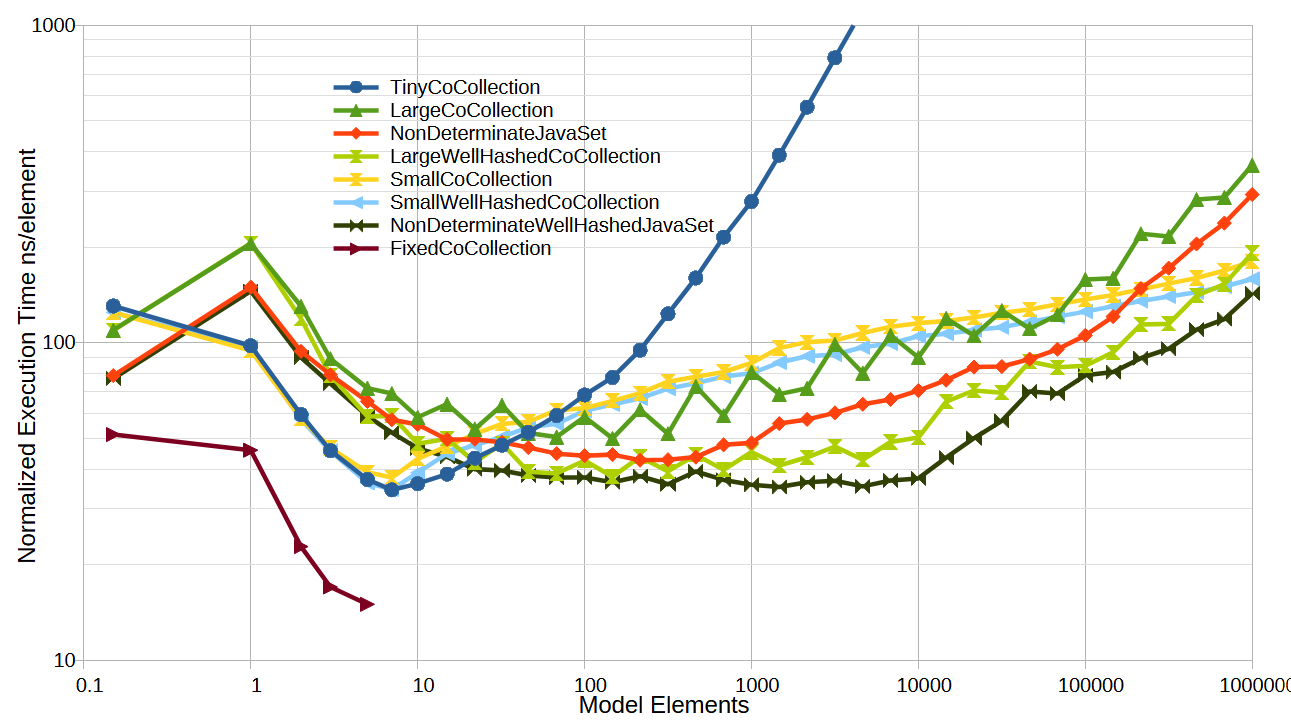
\includegraphics[width=6.0in]{ConstructionPlusIntersection.png}
	\end{center}
	\caption{Performances constructing two sets and an intersection}
	\label{fig:ConstructionPlusIntersection}
	\vspace{-20pt}
\end{figure}

The NonDeterminateJavaSet and NonDeterminateWellHashedJavaSet curves show the use of a Java HashSet without any attempt to maintain ordering; the performance is therefore not deterministic. For large collections the HashSet can be as much as four times faster than any of our \verb!CoCollection! approaches.

Two curves are shown since a distinctly better performance is achieved when perfect hash codes guarantee uniqueness. For Class-type elements for which the object address could provide a unique value, it might be expected that Java's System.identifierHashCode would be a good hash; it isn't. For the 'well-hashed' curves, the hash is allocated from an incrementing count, as could be achieved by a model loader/manager. The NonDeterminateJavaSet curve demonstrates far more hash table collisions than the NonDeterminateWellHashedJavaSet.

%Maintenance of a sorted order requires a reliable hash code. This is very simple for Class-type elements for which the object address provides a unique value. For simple PrimitiveType elements, the data value provides a distinctive value. It is only for composite DataTypes such as String, Collection and Tuple that the hashcode must be computed hierarchically. The hashcode can be cached to avoid redundant evaluation. In the case of a String, the hashcode is widely used, so it probably exists anyway.

The SmallCoCollection curves show a design expected to be suitable for small collections. It degrades steadily with size but is actually better than NonDeterminateJavaSet for huge models. It is much less sensitive to hashcode quality.

The TinyCoCollection curve uses an insertion rather than quick sort to prepare the \verb!hash2index! entry array. As expected, this is O(N*N) for larger collections. It is better than the SmallCoCollection below 50 model elements.

The LargeCollection augments the SmallCoCollection with a HashSet to accelerate look-ups as suggested by \cite{willink2017deterministic}. This helps significantly when the hash codes are perfect.

Finally the FixedCoCollection `curve' shows the performance of bespoke implementations for 0, 1, 2, 3 or 4 model elements. These are significantly faster through reduced overheads, but more significantly because there are no memory allocations for \verb!elements! or \verb!hash2index! arrays. The ` \verb!elements!' memory is realized on the stack where it avoids cache conflicts and may be cached in registers. Use of the \verb!hash2index! array is replaced by linear searches.

Small collections are very common, so clearly the FixedCoCollections can give determinism and a significant five-fold improvement over a Java HashSet.  Up to 20 model elements can be faster and deterministic with a TinyCoCollection. For larger collections the cost of determinism may be two-fold. Note that since OCL collections are immutable, choosing the optimum collection approach can be done prior to construction.

The CoCollection approach provides more opportunities for sharing, so the two source sets may already be available. It is therefore interesting to look at just the create-intersection cost. The corresponding performances are shown in Figure~\ref{fig:Intersection}. For really small collections, the FixedCoCollection gives determinism and a ten-fold improvement over a HashSet. For larger collections the Tiny or SmallCoCollection gives determinism and a two to three-fold improvement.

\begin{figure}
	\begin{center}
		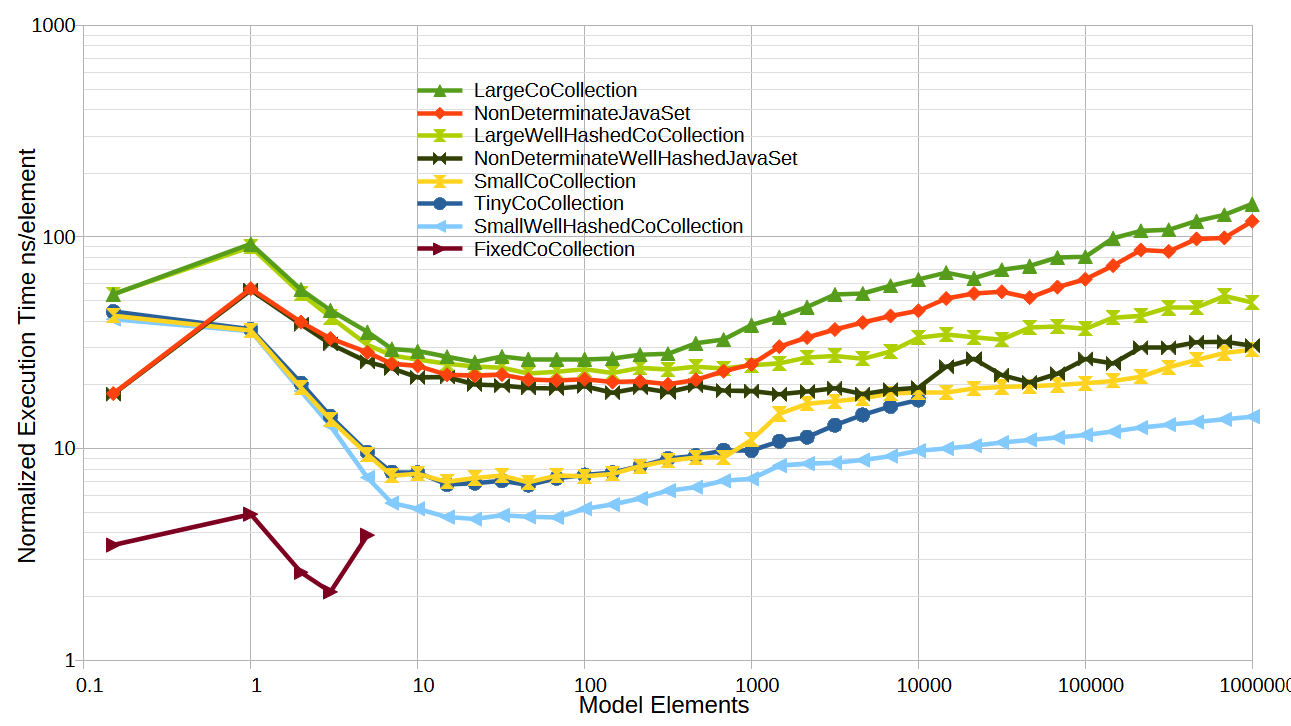
\includegraphics[width=6.0in]{Intersection.png}
	\end{center}
	\caption{Performances constructing an intersection}
	\label{fig:Intersection}
	\vspace{-20pt}
\end{figure}

%The problem as posed considered an isolated intersection using immutable variables. If however we consider an intersection that forms part of a larger OCL computation we may find that `ctor' and `init' costs can be shared with preceding terms.  The Java HashSet provides a good self-standing component, but there is no opportunity to share internal products. The new flat set exploits derived state that may be lazily computed and cached within the \verb!CoCollection!. The \verb!CoCollection! supports a neutral deterministic ordered content that may have multiple views. Thus when using a \verb!CoCollection!, \verb!aCollection->asSet! does not need to create a new HashSet with duplicate differently arranged content elements. Rather the original elements are re-used with the \verb!CoCollection! supporting the \verb!asSet! view. The new flat set as part of a \verb!CoCollection! offers significant opportunities for speed as well as space improvements. The extent of the improvements will be very dependent on the expressions in which collections are used and the ability of a compiler to exploit sharing.

The third paper \cite{Willink-Collections3} in this series exploits the \verb!CoCollection! representation to share computational effort across cascades of collection operations.

\section{Related Work}\label{Related Work}

Each of Dresden OCL \cite{Dresden-OCL}, Eclipse OCL \cite{Eclipse-OCL} and USE \cite{USE} pursue the same Java implementation approach for OCL collections; a family of kind-specific classes provides OCL semantics for a hidden internal representation using distinct Java classes, some standard, some bespoke. There is no sharing of a unified internal representation as proposed for the \verb!CoCollection!.

This work builds on the successes and remedies the failures of \cite{willink2017deterministic}.

Many authors \cite{wilke2011uml} have found aspects of the OCL specification worthy of criticism, but have held back, perhaps having too much respect for a specification that at its heart is obviously sensible.

This paper is perhaps unique in challenging the OCL 2.4 \S11.8 statement delegating semantics to `iterate'. Adherence to this statement imposes a procedural approach despite many operations such as \verb!select! being amenable to a declarative approach.  

OCL$\natural$ \cite{steimann2023ocl} uses \verb!iterate! as the sole mechanism for deconstruction.

\section{Summary}\label{Summary}

We have reformulated the implementations of the four collection kinds using lightweight kind-specific views of a shared unified deterministic ordered \verb!CoCollection!. Our results show that determinism can be provided with a threefold space saving, with a five-fold speed up for very small collections, and without speed penalty for collections of up to about 50 model elements and at moderate speed penalty for larger collections. Our results indicate a useful further speed-up when the sharing opportunities of \verb!CoCollection!s are exploited. Rather than a cost, there are functional benefits for making OCL deterministic. 

We have re-specified the iteration operations replacing the inadequate \verb!iterate! by fully-specified declarative \verb!gather! and procedural \verb!search!. The rewrites are suitable for implementation.

Normalization of collection expressions to one representation and two iterations paves the way for cascade operation in our third paper. 
%% The declaration on generative AI comes in effect
%% in Janary 2025. See also
%% https://ceur-ws.org/GenAI/Policy.html
\section*{Declaration on Generative AI}
  The author(s) have not employed any Generative AI tools.


%%
%% Define the bibliography file to be used
\bibliography{OCLCollections}

\end{document}
